\subsection{Co-Creation Workshops}

There were two workshops held with the Zambia coaches: one at the beginning of the week (before any app tests), and one at the end of the week (after all of the app tests). Below, the learning from these are presented.

\subsubsection{Co-Designing an App for the YoungDrive Training}

    The result was fantastic, in the sense that it gave an unbiased look at what the coaches expected from the app, what functionality wasn't important, and into their technical preferences. A simpler design than originally thought was deemed sufficient, and the simple sketches guided continued development of the app during the week. From using the devices, it was found that most coaches prefer using the tablet (5 for tablet, versus 2 for smartphone and 2 for computer). Both the designs and insights gained were used throughout the week to further improve the simple app created at the end of iteration 1. The workshop gave great insights to who the coaches were and their thinking.

    \subsubsection{Understanding what Builds Confidence among Coaches}

    During this workshop, the focus was to examine what builds confidence among the coaches. The following clusters could be determined: "I believe in myself" (3 coaches), "I believe in God" (2 coaches), "I am well prepared" (4 coaches) and "I am certified" (1 coach). See figure \ref{fig:zambiaWorkshop2} for the different clusters. Josefina comments after the workshop: “I have a problem: There is no way I can control them how they have prepared themselves for a youth session.", says Josefina.

    \begin{figure}[h]
        \centering
        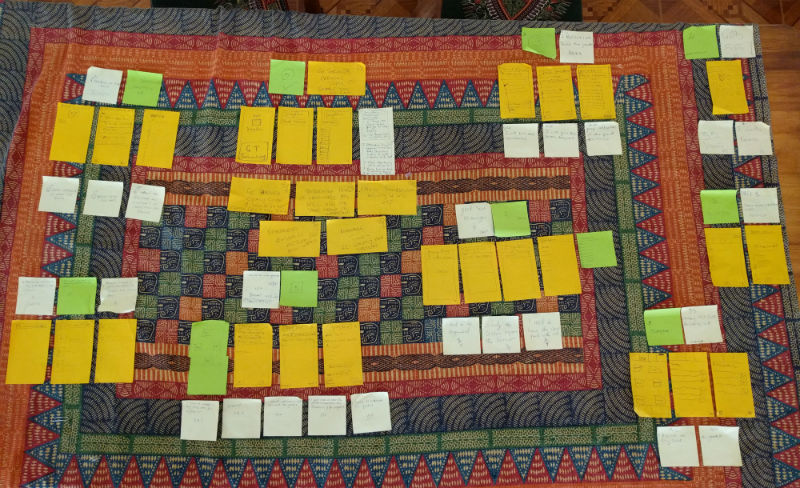
\includegraphics[width=0.9\textwidth]{zambiaWorkshop2small.jpg}
        \caption{The clustered postits with needs, together with included design proposals.}
        \label{fig:zambiaWorkshop2}
    \end{figure}
